
\documentclass[xcolor=dvipsnames, compress, t]{beamer}

\usetheme{CambridgeUS}
\usepackage[english]{babel}
\usepackage{color}
\usepackage{graphics}
\usepackage{graphicx}
\usepackage{stmaryrd}
\usepackage{etoolbox}
\usepackage{multicol}
\usepackage{tikz}
\usetikzlibrary{shapes.geometric, arrows}
\usepackage{booktabs}


\usepackage{dsfont}
\usepackage{etoolbox}
\usepackage{accents}
\usepackage{sgame}
\usepackage{epstopdf}
\usepackage{wrapfig}
\usepackage{tabto}

\setbeamertemplate{theorems}[numbered]
\undef{\lemma}
\newtheorem{lemma}{\translate{Lemma}} %gives own numbered lemmas
\newtheorem{prop}{Proposition}
\newtheorem{defin}{Definition}
\newenvironment{sketch}[1][Sketch of Proof.]{ \begin{trivlist} \item[\hskip \labelsep {\bfseries #1}]}{\end{trivlist}}

%colors

\definecolor{NIUred}{RGB}{200,16,46 } 
\definecolor{NIUblack}{RGB}{0,0,0}
\definecolor{NIUpantone}{RGB}{165,167,168}

\setbeamercolor{palette primary}{bg=NIUblack,fg=white}
\setbeamercolor{palette secondary}{bg=NIUpantone,fg=white}
\setbeamercolor{palette tertiary}{bg=NIUred,fg=white}
\setbeamercolor{palette quaternary}{bg=NIUred,fg=white}
\setbeamercolor{structure}{fg=NIUred} % itemize, enumerate, etc
\setbeamercolor{section in toc}{fg=NIUred} % TOC sections
%\setbeamercolor{subsection in head/foot}{bg=NIUpantone,fg=white}
%%Special Commands
\newcommand\munderbar[1]{%
	\underaccent{\bar}{#1}}

\newcommand{\der}{\mathrm{d}}
\newcommand{\e}{\mathrm{e}}

\newcommand{\vs}{\vspace{\baselineskip}}
\newcommand{\vf}{\vspace{5pt}}
\newcommand{\draw}{{\color{Plum} \bf Drawing.}} 
%use this if there is a drawing that you can't include
\newcommand{\wts}[1]{{\color{Orchid} \textbf{\underline{WTS}:}  #1}} 
%use this for what to show!

\setbeamertemplate{navigation symbols}{} 
\setbeamertemplate{enumerate items}[default]

%%Don't change things above this%%

%%%%%%%%%%%%%%%%%%


\title[691 Presentation]{Demographics and U.S. Presidential Elections}

\subtitle{Can Changing Population Characteristics Explain Elections?}

\author{Ethan Rahman}
\institute[NIU]{\vspace{-10pt} \large Northern Illinois University}
\date{October 15, 2021}

\renewcommand{\thedefin}{4.\Alph{defin}} %ended on 4.C
\setcounter{defin}{3}

\renewcommand{\thetheorem}{4.\arabic{theorem}} %ended on 4.2
\setcounter{theorem}{2}

\renewcommand{\thelemma}{4.\roman{lemma}}
\setcounter{lemma}{0}

\begin{document}
	\begin{frame}
		\titlepage
	\end{frame}
	
	\begin{frame}{States} 
		I was assigned 5 states in the mid-Atlantic region of the United States:
		\begin{minipage}{.25 \textwidth}
			\begin{itemize}
				\item Maryland
				\item Pennsylvania
				\item New Jersey
				\item Virginia
				\item Delaware
			\end{itemize}
		\end{minipage}
		\begin{minipage}{.50\textwidth}
			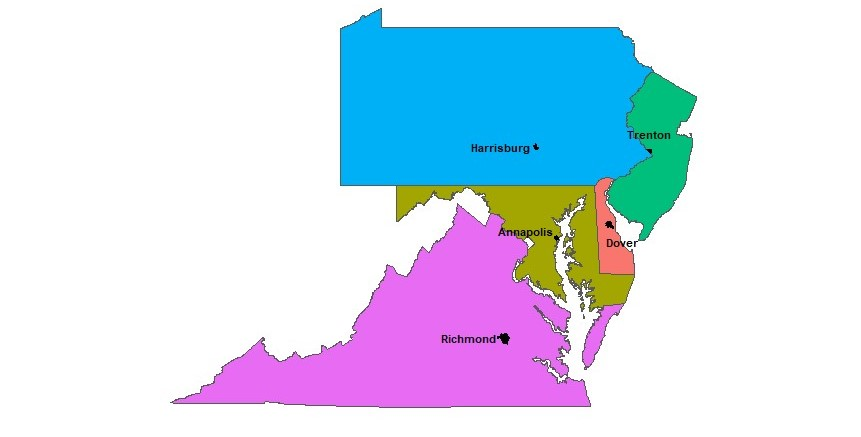
\includegraphics[width=1.8\textwidth]{Rplot03_cropped.jpg}
		\end{minipage}
	\end{frame}
	\begin{frame}{Brief Overview of Each State} 
		\begin{center}
			
			\begin{table}
				\resizebox{\textwidth}{!}{%
					\begin{tabular}{ |p{0.16\linewidth}|p{0.12\linewidth}|p{0.18\linewidth}|p{0.18\linewidth}|p{0.18\linewidth}|p{0.16\linewidth}| } 
						\hline
						\multicolumn{6}{|c|}{Mid Atlantic States}		\\
						\hline
						{}           & Maryland & Pennsylvania & New Jersey & Virginia & Delaware\\
						\hline 
						Population   & 6,018,848& 12,791,530   & 8,878,503  & 8,454,463&  957,248\\ 
						Largest City &Baltimore & Philadelphia &Newark  &Virginia Beach& Wilmington\\ 
						Largest Industry (by number of employees) & Real estate&Health Care and Social Assistance &Health Care and Social Assistance & Health Care and Social Assistance & Finance and insurance \\
						\hline
				\end{tabular}}
				\label{}
				\caption{https://www.bls.gov/oes/tables.htm}
			\end{table}
			
			
		\end{center}	
	\end{frame}
	
	\begin{frame}{Voting Patterns}
		From 2016 to 2020, there have been clear shifts in the number of votes recieved by the two major candidates for the US Presidential Election.
		\begin{figure}[1]
			\centering
			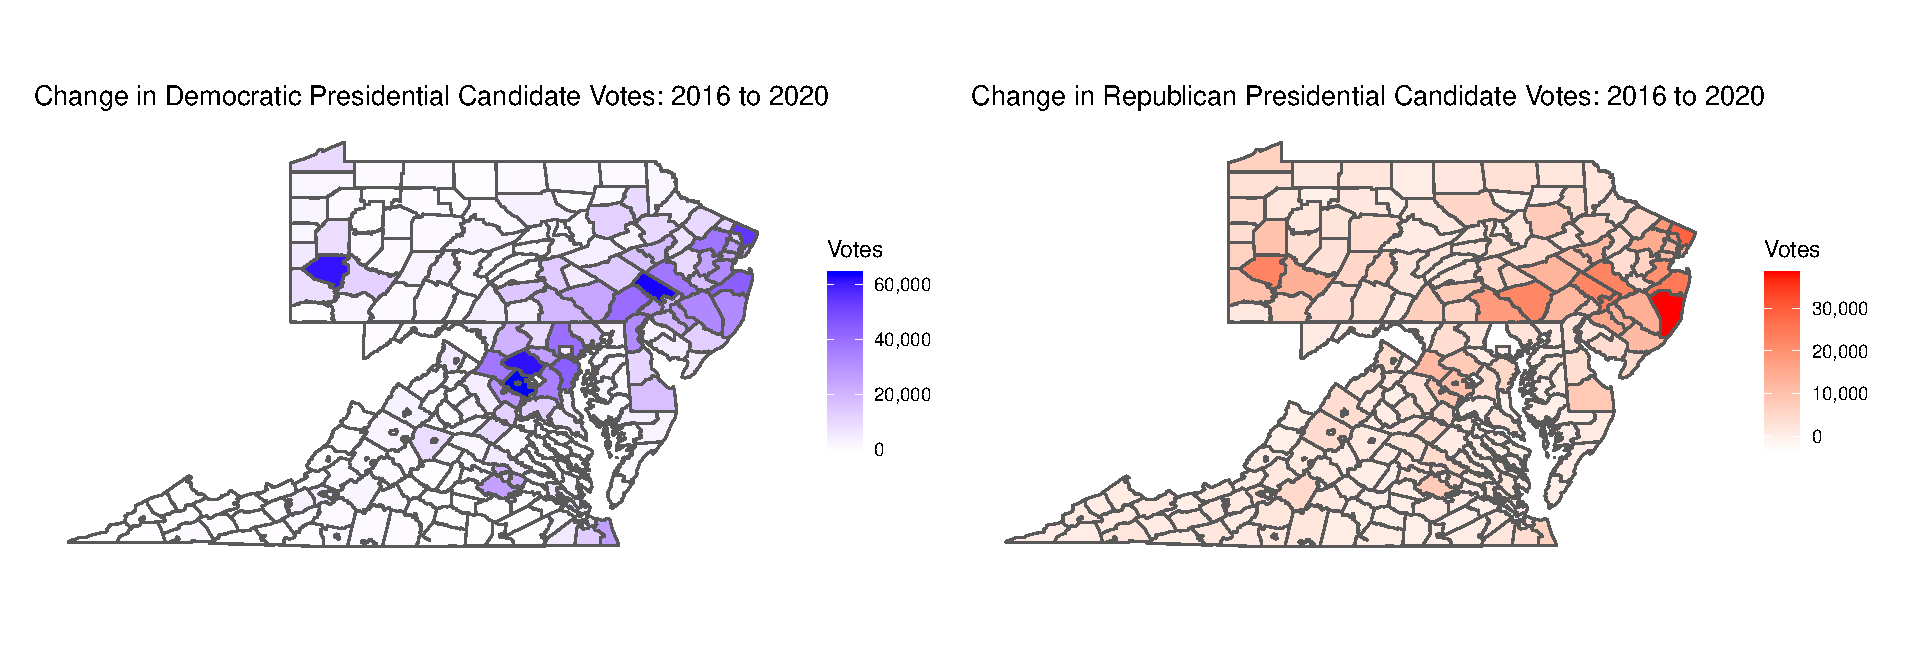
\includegraphics[width=1\textwidth]{vote_changes.eps}
			\caption{Some of these changes could be explained by population growth, or changes in voter participation. To what extent can demography illustrate a fuller picture?}
		\end{figure}
	\end{frame}
	\begin{frame}
		\begin{minipage}{.50\linewidth}
			peepee
		\end{minipage}
		\begin{minipage}{.40\linewidth}
			% Table generated by Excel2LaTeX from sheet 'Sheet1'
\UseRawInputEncoding
\begin{table}[htbp]
  \centering
  \caption{Add caption}
  \resizebox{\textwidth}{!}{%
    \begin{tabular}{p{6.11em}p{11.835em}}
    \toprule
    \multicolumn{1}{l}{} & \textit{Dependent variable:} \\
    \multicolumn{1}{r}{} & \multicolumn{1}{r}{} \\
\cmidrule{2-2}    \multicolumn{1}{l}{} & vote\_change.REPUBLICAN \\
    \multicolumn{2}{r}{} \\
    \midrule
    perMale2019 & \multicolumn{1}{r}{25,679.63} \\
    \multicolumn{1}{l}{} & \multicolumn{1}{r}{-43,206.67} \\
    \multicolumn{1}{l}{} & \multicolumn{1}{r}{} \\
    perWhite2019 & \multicolumn{1}{r}{-37,033.76} \\
    \multicolumn{1}{l}{} & \multicolumn{1}{r}{-29,214.96} \\
    \multicolumn{1}{l}{} & \multicolumn{1}{r}{} \\
    Constant & 3,594.208*** \\
    \multicolumn{1}{l}{} & \multicolumn{1}{r}{-384.436} \\
    \multicolumn{1}{l}{} & \multicolumn{1}{r}{} \\
    \multicolumn{2}{r}{} \\
    \midrule
    Observations & \multicolumn{1}{r}{248} \\
    R2    & \multicolumn{1}{r}{0.01} \\
    Adjusted R2 & \multicolumn{1}{r}{0.002} \\
    Residual Std. Error & 5,679.760 (df = 245) \\
    F Statistic & 1.192 (df = 2; 245) \\
    \multicolumn{2}{r}{} \\
    \midrule
    Note: & *p<0.1;�**p<0.05;�***p<0.01 \\
    \end{tabular}}%
  \label{tab:addlabel}%
\end{table}%

		\end{minipage}
	\end{frame}
\end{document}